\section{Experimental Validation}
\label{sec:experiment}
\label{sec:experimental_design}
\label{sec:experimental_validation}

In order to subject our theory to an experimental test,
  we use the IIMB dataset\footnote{\URL{islab.di.unimi.it/iimb}}
  used in the instance matching track of the
  2012 Ontology Alignment Evaluation Initiative
  (OAEI)\footnote{\URL{oaei.ontologymatching.org}}.
This dataset consists of eighty ontologies $G_i$ (for $1 \leq i \leq 80$)
  that are linked to a single base ontology $G_0$.
The identity links between $G_0$ and $G_i$ are annotated with a
  confidence measure between $0.0$ and $1.0$.
A graph $G$ is the result of fully materializing the graph merge
  of $G_i$ (for some $1 \leq i \leq 80$) and $G_0$.
For each of these eighty linked ontologies a reference mapping is available.

In our experiment we ran separate tests for each of the $80$ datasets
  and took the average values for incremental reductions of
  random parts of the identity relations between $G_0$ and the $80$
  different $G_i$'s.
In other words: we deliberately make the identity relation incomplete.
We then calculate the rough set representation using this altered relation.
Subsequently ,we evaluate how many of the removed identity pairs occur in
  the higher approximation.
Our hypothesis is that the percentage of removed \emph{identity pairs}
  in the higher approximation is larger than the percentage of \emph{pairs}
  in the higher approximation.
If the hypothesis is validated, this indicates that
  calculating the rough set representation for a partial identity relation
  would indeed improve suggestions for extending that identity relation.

Since the data may contain noise, using precision degrees $0.0$ and $1.0$
  may be too strict. For this experiment we have set the boundaries
  to $0.05$ and $0.95$ respectively.

Figure \ref{fig:recall_quality} shows the different behaviors of the
  upper and lower approximations, with the upper approximation indeed
  having a dramatically higher recall than the lower approximation.

\begin{figure}
\centering
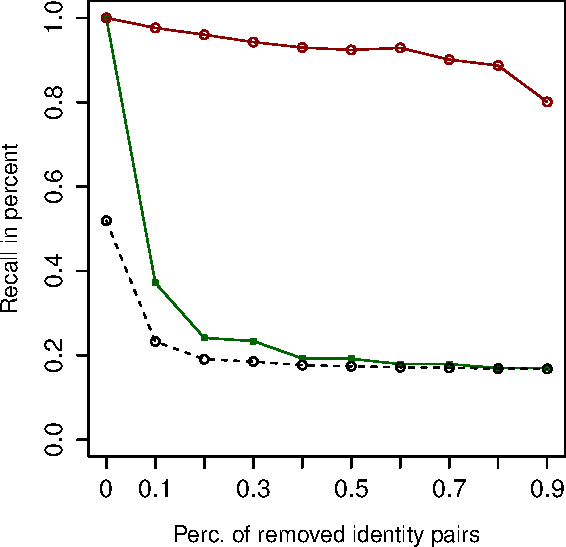
\includegraphics[width=0.8\linewidth]{./img/recall_quality}
\caption{
  The recall of the lower and higher approximation
    is shown by the green line (circles) and red line (boxes) respectively.
  The quality metric (definition \ref{def:quality})
    is shown by the dashed line.
}
\label{fig:recall_quality}
\end{figure}

In figure \ref{fig:in_higher}
  we see that the randomly removed identity pairs are often
  in the higher approximation, even when large parts of
  the identity relation are removed.

\begin{figure}
\centering
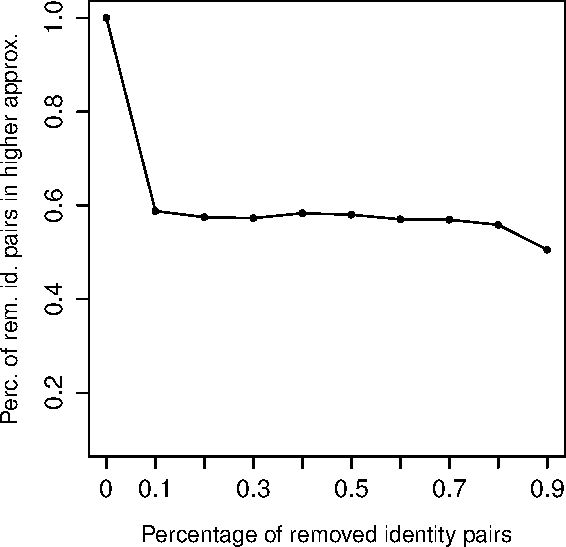
\includegraphics[width=0.8\linewidth]{./img/in_higher}
\caption{
  The percentage of the removed identity pairs that are in the higher approximation
}
\label{fig:in_higher}
\end{figure}

\begin{comment}
Lower recall
1.0,0.37172100183246687,0.24123550044617229,0.23375413992878838,0.19251810221158194,0.1916729296953922,0.1790536768898471,0.17912482945205316,0.1696252362320524,0.17011849853438268
Higher recall
1.0,0.976185052819561,0.9600384749021372,0.9425765362723856,0.9297564861502547,0.9239282325982691,0.9288077551757412,0.900878631549093,0.886987450993775,0.8005503359226204
Quality
0.5190405227795084,0.23261438049447705,0.1904353344556299,0.18505145463363135,0.17658153004935476,0.17387635867899948,0.17168948193128328,0.17017370794837366,0.16844506704419984,0.1677780567227606
Higher cover
0.0006413304103753317,0.0006098495555258293,0.0005825544051162525,0.0005747252831024628,0.0005640718998200667,0.0005626590987592347,0.0005613753926606205,0.0005464403973849621,0.0005372610299329459,0.00046916805031848495
Removed identity pairs in higher
1.0,0.5877680311890837,0.5747530425162004,0.572660333493667,0.5831761670185315,0.5799385908868745,0.5701984042084377,0.5692284399224807,0.558405393333526,0.5051324217787632
\end{comment}



\subsection{Future Experiments}
\label{sec:hypotheses}

Space limitations do not allow us to describe the results of further
  experiments. Instead, we will describe some of the other hypotheses
  that can be evaluated using our approach:
\begin{enumerate}
\item Take an {\small \texttt{owl:sameAs}} relation and
        a {\small \texttt{skos:related}}
        relation defined over the same domain.
      Merge them into a new binary relation $\sim$.
      Establishing the lower and higher approximation of $\sim$,
        the hypothesis is that pairs from {\small \texttt{owl:sameAs}}
        occur more frequently in the lower boundary than pairs from
        {\small \texttt{skos:related}},
\item Take a set of alignment pairs, each associated with a confidence measure
        between $0.0$ and $1.0$.
      Choose an arbitrary cutoff point $0.0 < c < 1.0$.
      The hypothesis is that alignments with a confidence larger than $c$
        occur more frequently in the lower approximation than alignments
        with a confidence smaller than $c$.
\item Take a set of automatically generated alignment pairs with
        associated confidence measures and take the gold standard or
        reference alignment for the same dataset.
      The hypothesis is that pairs that occur in the lower approximation
        of the alignment appear relatively more often in the gold standard
        than pairs that occur in the higher approximation of the alignment.
\item The quality measure $\alpha$ of a reference alignment is generally
        higher than the accuracy measure of an automatically generated
        alignment for the same dataset.
      Or, the quality measure is generally higher for identity relations
        that domain experts consider to be correct.
\end{enumerate}

\noindent Finally, the IIMB datasets are quite small
  (tens of thousands of triples).
We will have to verify whether the current implementation is able to scale
  to bigger datasets.
